\documentclass[14pt, russian]{article}
\usepackage{graphicx}
\usepackage[a4paper,left=2.5cm,right=2.5cm,top=2.5cm,bottom=2.5cm]{geometry}%
\linespread{1.3}
\usepackage{amsbsy}
\usepackage{amssymb}
\usepackage[T2A]{fontenc}
\usepackage[cp1251]{inputenc}
\usepackage[russian]{babel}
\usepackage{epstopdf}
\usepackage[autostyle]{csquotes}
\usepackage{cuted}   
\usepackage{lipsum}  
\usepackage[intoc,nocfg,russian]{nomencl}
\newcommand{\nomencl}[2]{#1 --- #2\nomenclature{#1}{#2}}
\setlength{\nomlabelwidth}{3em}
\setlength{\nomitemsep}{-\parsep}
\setcounter{tocdepth}{2}
\renewcommand{\nomlabel}[1]{#1 ---}
\makenomenclature
\usepackage{wrapfig}
\let\vec=\mathbf
\def\mprp{\mbox{\tiny $\bot$}}
\def\mprl{\mbox{\tiny $\|$}}
\def\th{\mbox{th}}
\def\D{\mathrm{d}}
\def\beq{\begin{eqnarray}}
\def\eeq{\end{eqnarray}}
\def\ee{\varepsilon}
\def\lm{\lambda}
\newcommand{\ii}{\mathrm{i}} % мнимая единица
\newcommand{\dd}{\mathrm{d}} % дифференциал
\newcommand{\eee}{\mathrm{e}} % основание натуральных логарифмов

\newcommand{\bs}{\boldsymbol}

\begin{document}

%%%%%%%%%%%%%%%%%%%%%%%%%%%%%%%%%%%%%%%%%%%%%%%%%%%%%%%%%%%%%%%%%%%%%%%%

\title{Затухание фотона в замагниченной плазме}
\author{Д.А. Румянцев, А.А. Ярков, Д.М. Шленев}
\date{}
\maketitle


\section{Введение}

Как известно, в присутствии сильно замагниченной среды 
возможны изменения дисперсионных и поляризационных свойств фотонов (см., например,~\cite{KuznMikh}). Этот факт 
может приводить к существенным изменениям кинематики процессов, в результате 
которых, например, становятся возможными такие одновершинные реакции, как однофотонное 
рождение электрон-позитронной пары $\gamma\to e^+e^-$ или поглощение фотона 
$e^{\pm}\gamma\to e^{\pm}$, которые кинематически запрещены или подавлены в 
вакууме. Однако, в выражениях для этих процессов присутствуют сингулярности, которые связаны со свойствами фазовых объемов древесных процессов (см., например,~\cite{Klepikov:1954,Sturrock:1971,Tademaru:1973,Daugherty:1983,Shabad:1988}). В связи с этим возникает принципиально важная задача физически корректного определения коэффициента поглощения вблизи окрестностей этих сингулярностей, соответствующих резонансным областям. При расчетах физических величин все резонансные бесконечные пики усреднялись~\cite{Baier:2007}, что позволило получить конечные результаты, однако такой подход не устраняет сингулярности, поэтому требуется переформулировать модель в других терминах.

Для этого в работе~\cite{Shabad:1988} предлагалось рассматривать фотон как затухающую электромагнитную волну, то есть исследовать временную зависимость волновой функции фотона. Изначально подобная задача в классическом варианте рассматривалось в работе~\cite{Landau:1946} для бесстолкновительной плазмы (т.н. затухание Ландау). Если в классической задаче затухание связано либо с передачей энергии электромагнитного поля частицам, движущимся в фазе с волной, либо с ларморовым вращением частиц, то в квантовой электродинамике затухание квантованной электромагнитной волны определяется квантовыми процессами поглощения и рождения фотонов. Это непосредственно связано с обратимостью как классических, так и квантовых процессов, определяющих затухание.

Для поиска временной зависимости волновой функции фотона в работе~\cite{Shabad:1988} предлагалось решать уравнение дисперсии на втором римановом листе. Однако как было отмечено в работе~\cite{MikhChist:2001}, такой метод имеет ряд недостатков. Во-первых, решения с комплексными энергиями фотона находятся на нефизических римановых листах, количество которых вообще говоря бесконечно. Это приводит к возникновению бесконечного числа решений уравнения дисперсии как с положительными, так и с отрицательными значениями мнимой части энергии. Во-вторых, в данном методе в околопороговой области предполагался экспоненциальный характер затухания электромагнитной волны, что, вообще говоря, согласно выводам авторов~\cite{MikhChist:2001}, не так. Поэтому в работе~\cite{MikhChist:2001} для исследования временного затухания электромагнитной волны во внешнем магнитном поле был рассмотрен метод, который заключается в нахождении запаздывающего решения уравнения электромагнитного поля в присутствии внешнего источника с учетом поляризации вакуума во внешнем магнитном поле. С другой стороны, в работе~\cite{MikhChist:2001} неэкспоненциальное затухание фотона рассматривалось в приближении сильного магнитного поля, когда все электроны и позитроны занимают основной уровень Ландау, однако в случае замагниченной плазмы таких исследований не проводилось, что является актуальным, поскольку для астрофизических приложений наличие замагниченной среды является наиболее характерным фактором.

%%%%%%%%%%%%%%%%%%%%%%%%%%%%%%%%%%%%%%%%%%%%%%%%%%%%%%%%%%%%%%%%%%%%%%%%%%%%%%%%%%%%%%%%%%%%%%%%%%%%%%%%%%%%%%%%%%%%%%%%%%%%%%%%%%%%%%%%%%%%%%%%%%%%%%%%%%%
\section{Распространение фотона в замагниченной среде}

Для описания эволюции электромагнитной волны ${\cal A}_{\alpha}(x)$, где $x_\mu = (t, {\bf x})$ в замагниченной плазме, 
во времени воспользуемся методикой, подробно изложенной в~\cite{MikhChist:2001} для случая магнитного поля. Данная методика заключается в определении реакции системы 
(${\cal A}_{\alpha}(x)$ и замагниченной плазмы) на внешний источник~\cite{Kirzhnits:1987}, создающий начальное состояние, который адиабатически включается 
при $t = - \infty$ и в момент времени $t = 0$ выключается. При $t > 0$
электромагнитная волна в плазме будет эволюционировать самостоятельно. Для простоты будем рассматривать эволюцию монохроматической волны, поэтому 
функцию источника удобно выбрать в том же виде, что и для сильного магнитного поля:
%
\beq
{\cal J}_{\alpha}(x) = j_{\alpha}\,e^{i \,{\bf k} {\bf x}}\,
e^{ \varepsilon t}\, \theta(- t), \,\,\, \varepsilon \to 0^+,
\label{eq:1}
\eeq
где 4-мерный вектор тока удобно выбрать следующим образом: $j_{\alpha} = (0, {\bf j})$. В этом случае закон сохранения тока --  ${\bf j} \cdot {\bf k} = 0$.  Зависимость ${\cal A}_{\alpha}(x)$ от времени  определяется уравнением
%
\begin{eqnarray}\label{eq:WaveEq}
%\nonumber
%&& 
(g_{\alpha \beta} \, \partial_{\mu}^2  -
\partial_{\alpha}\partial_{\beta}) \, {\cal A}_{\beta}(x) + 
%\nonumber \\
%&&+ 
\int d^4 x'\, {\cal P}_{\alpha \beta} (x - x') \, {\cal A}_{\beta}(x')
= {\cal J}_{\alpha}(x),
\label{eq:2}
\end{eqnarray}
где ${\cal P}_{\alpha \beta} (x - x')$ -- поляризационный оператор фотона в магнитном поле и плазме. $q^{\mu} = (q_0,\, {\bf k})$ -- 4-вектор импульса фотона.


Запаздывающее решение уравнения~(\ref{eq:WaveEq}) можно представить в следующем виде:

\begin{equation}\label{eq:RetSol}
	{\cal A}_\alpha(x)=\int \dd^4 x' G^R_{\alpha \beta}(x-x'){\cal J}_\beta(x')\, ,
\end{equation}
где $G^R_{\alpha \beta}(x-x')$ -- запаздывающая функция Грина (см., например~\cite{Landau:2001}).

Следуя работе~\cite{MikhChist:2001}, аналогично процессу затухания в магнитном поле, воспользуемся следующим соотношением между запаздывающей $G^R_{\alpha\beta}(x-x')$ и причинной $G^C_{\alpha\beta}(x-x')$ функциями Грина:

\begin{equation}\label{eq:RetCasualGreen}
G^R_{\alpha\beta}(x-x')= 2 \mathrm{Re} \left[G^C_{\alpha\beta}(x-x')\right]\theta(t-t')\, .
\end{equation}

\begin{center}
	\begin{figure}[t!]\centering
		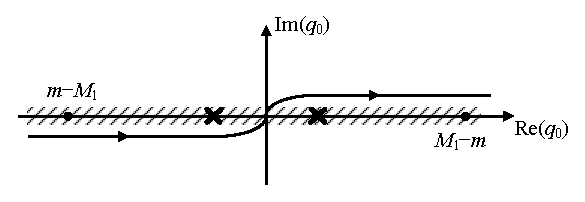
\includegraphics[scale=1.5]{Fig1.eps}
		\caption{Контур интегрирования по $q_0$ в~(\ref{eq:FullIntegrate}) для моды 1. Штрихами показана область нестабильности фотона. Крестиком обозначен полюс, соответствующий $q_0=\omega$ -- вещественному собственному значению поляризационного оператора, точками обозначены полюса.} \label{fig:FullPathIntegrMode1}
	\end{figure}
\end{center}

Поляризационные и дисперсионные свойства фотона определяются поляризационным оператором фотона ${\cal P}_{\alpha\beta}$, явный вид которого может быть получен из результатов работ~\cite{Shabad:1988,Tsai:1974,Batalin:1971,Skobelev:1975}. Его удобно разложить по собственным векторам $r^{(\lambda)}_\alpha$ и собственным значениям ${\cal P}^{(\lambda)}$:
%
\begin{equation}
\label{eq:Pab10}
{\cal P}_{\alpha \beta} = \sum_{\lambda = 1}^{3} 
{\cal P}^{(\lambda)} \, \frac{r_{\alpha}^{(\lambda)} 
	(r_{\beta}^{(\lambda)})^{*}}{(r^{(\lambda)})^2}\, . 
\end{equation}
%

В случае сильно замагниченной плазмы $\beta = eB \gg T^2$ и $\mu=0$ собственные векторы поляризационного оператора фотона приближенно будут такими же, как и в чистом магнитном поле (подробный анализ дисперсионных свойств фотона в замагниченной среде можно найти в работе~\cite{Chistyakov:2009} и цитированных в ней статьях):
%
\begin{equation}
\label{eq:r12}
r^{(1)}_{\alpha} \simeq  -2 q^2_{\mprp} \, (\varphi q)_\alpha\,, \qquad r^{(2)}_{\alpha} \simeq (\tilde\varphi q)_\alpha \, ,
\end{equation}
%
где $\varphi_{\mu \nu} =  F_{\mu \nu} /B$ -- обезразмеренный тензор электромагнитного поля и ${\tilde \varphi}_{\mu \nu} = \frac{1}{2}\varepsilon_{\mu \nu \rho \sigma} \varphi_{\rho \sigma}$ -- тензор, дуальный к нему, а также введены обозначения $q_{\mprp}^2 = q_x^2 + q_y^2$, $q_{\mprl}^2 = q_0^2 - q_z^2$.

Соответствующие этим модам собственные значения поляризационного оператора имеют вид:
%
\begin{equation}
\label{eq:kappa10}
{\cal P}^{(1)} \simeq \frac{\alpha}{3\pi} \, q^2 \, {\cal V} - \frac{\alpha}{3\pi} \, 
q^2_{\mprp}\, ,
\end{equation}
%
\begin{equation}
\label{eq:kappa2}
{\cal P}^{(2)} = \frac{\alpha}{3\pi} \, q^2 \, {\cal V} + \frac{2 \alpha}{\pi} \, \beta \, {\cal D} \, ,
\end{equation}
%
\begin{equation}
\label{eq:Lambda}
{\cal V} = \ln{(B/B_e)} - 1.792 + \frac{3}{2} \, \int\limits_0^1 \dd x \, (1-x^2) \, 
\ln{\left [1- \frac{q^2}{4m^2} \, (1-x^2) \right ]} \, .
\end{equation}
%
\begin{equation}
\label{eq:PabD}
{\cal D} = - {\cal J}_1 (q_{\mprl})  - 
H \left (\frac{q^2_{\mprl}}{4m^2} \right)  \, , 
\end{equation}
%
\begin{equation}
\label{eq:PabJ}
{\cal J}_1 (q_{\mprl}) = 2q^2_{\mprl} \, m^2 \, \int\limits_{-\infty}^{\infty}  \frac{\dd p_z}{E} \, 
\frac{f_{-}(p) + f_{+}(p)}{q_{\mprl}^4 - 4(pq)^2_{\mprl}} \, , 
\end{equation}
%
\begin{eqnarray}
\label{eq:H0}
%\nonumber
H(z)&=&\frac{1}{\sqrt{z(1 - z)}} \, \arctg \sqrt{\frac{z}{1 - z}} - 1,
\quad 0 \leqslant z \leqslant 1,
\\ [3mm]
\label{eq:H1}
H(z) &=& - \frac{1}{2\sqrt{z(z-1)}}
\ln  \frac{\sqrt{z} + \sqrt{z-1}}{\sqrt{z} - \sqrt{z-1}}  - 1 + 
\\[3mm]
\nonumber
&+& \frac{i\pi}{2\sqrt{z(z-1)}}, \quad z > 1, 
\end{eqnarray}

Разложение функции Грина по собственным векторам 
$r_\alpha^{(\lambda)}$ поляризационного оператора в замагниченной плазме 
выглядит следующим образом:
\begin{equation}\label{eq:InvGcFourier}
	G^C_{\alpha\beta}(x)=\int \frac{\dd^4q}{(2\pi)^4}G^C_{\alpha \beta}(q) e^{-\ii qx}\, ,
\end{equation}
\begin{equation}\label{eq:GcFourier}
	G^C_{\alpha\beta}(q)=\sum_{\lambda=1}^{3}\frac{r_\alpha^{(\lambda)}r^{(\lambda)}_\beta}{(r^{(\lambda)})^2}\cdot \frac{1}{q^2-{\cal P}^{(\lambda)}(q)}\, ,
\end{equation}

Вообще говоря, в замагниченной плазме из-за наличия анизотропии решение задачи о распространении фотона под произвольным углом к магнитному полю представляет значительные трудности. Поэтому, в качестве упрощения, рассмотрим частный случай, когда фотон распространяются поперек магнитного поля так, что $k_z=0$.
С учетом этого замечания, подставляя выражение~(\ref{eq:RetSol}) в (\ref{eq:WaveEq}) и используя~(\ref{eq:RetCasualGreen})--(\ref{eq:GcFourier}), получим следующий результат:
\begin{equation}\label{eq:ASolvePlasma}
	{\cal A}_\alpha(x) = 2 e^{i \mathbf{kx}} \mathrm{Re} \sum_{\lambda=1}^3 \int\frac{\dd q_0}{2\pi i}\frac{r_\alpha^{(\lambda)}(r^{(\lambda)} j)}{(r^{(\lambda)})^2}\frac{e^{-i q_0 t}}{(q_0-i\varepsilon)(q_0^2-\mathbf{k}^2-{\cal P}^{(\lambda)}(q))}\, .
\end{equation}

С учетом~(\ref{eq:r12}--\ref{eq:kappa2}) перепишем~(\ref{eq:ASolve}) в виде:

\begin{equation}\label{eq:ASolve}
	{\cal A}_\alpha(x) \simeq 2 e^{i \mathbf{kx}} \mathrm{Re} \sum_{\lambda=1}^3 \int\frac{\dd q_0}{2\pi i}\frac{\varepsilon_\alpha^{(\lambda)}(\varepsilon^{(\lambda)} j)}{(\varepsilon^{(\lambda)})^2}\frac{e^{-i q_0 t}}{(q_0-i\varepsilon)(q_0^2-\mathbf{k}^2-{\cal P}^{(\lambda)}(q))}\, .
\end{equation}

В силу линейного характера уравнения~(\ref{eq:WaveEq}), решение~(\ref{eq:ASolve}) для двух возможных поляризаций можно представить в виде:
\begin{equation}\label{eq:ASoveDivide}
	{\cal A}_\alpha(x)={\cal A}^{(1)}_\alpha(x)+{\cal A}^{(2)}_\alpha(x)\, ,
\end{equation}
где 
%
\begin{eqnarray}                        		
{\cal A}^{(\lambda)}_{\alpha} (x) = V^{(\lambda)}_\alpha (0, {\bf x}) \, Re F^{(\lambda)} (t) \, ,
\label{eq:V}
\end{eqnarray}
\begin{eqnarray}
V^{(\lambda)}_\alpha (0, {\bf x}) = 2\, e^{ i\, {\bf k x}} \, 
\varepsilon^{(\lambda)}_\alpha \, (\varepsilon^{(\lambda)} j)\, .
\label{eq:partialV}
\end{eqnarray}

Как следует из~(\ref{eq:ASoveDivide}) и~(\ref{eq:ASolve}) характер распространения фотона в сильно замагниченной плазме будет полностью определяться функцией $F^{(\lambda)} (t)$, которую удобно представить в виде Фурье-интеграла

\begin{equation}\label{eq:FullIntegrate}
	F^{(\lambda)}(t)=\int_C\frac{dq_0}{2\pi \ii}\frac{e^{-\ii q_0 t}}{(q_0-\ii \varepsilon)(q_0^2-\vec{k}^2-{\cal P}^{(\lambda)}(q))}.
\end{equation}

	\begin{figure}[t]\centering
		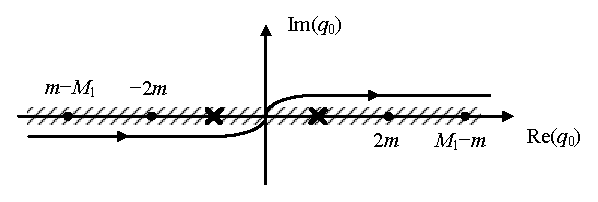
\includegraphics[scale=1.5]{Fig2.eps}
		\caption{Контур интегрирования по $q_0$ в~(\ref{eq:FullIntegrate}) для моды 2. Штрихами показана область нестабильности фотона. Крестиком обозначен полюс, соответствующий $q_0=\omega$ -- вещественному собственному значению поляризационного оператора.}\label{fig:FullPathIntegr}.
	\end{figure}

Контур интегрирования $C$ определяется согласно аналитическим свойствам подынтегрального выражения. В частности, в точке $q_0=\omega$ подынтегральное выражение~(\ref{eq:FullIntegrate}) имеет полюс, который соответствует уравнению дисперсии:

\begin{equation}
	\omega^2 - \vec{k}^2 - {\cal P^{(\lambda)}}(q)=0.
\end{equation}

С другой стороны, как было показано в работе~\cite{MikhChist:2001}, собственные значения поляризационного оператора как в магнитном поле, так и в замагниченной плазме помимо полюсов $q_{\mprl}^2=(M_n\pm M_\ell)^2$, также имеют разрезы, которые связаны с распадом фотона на $e^+e^-$-пару и переходом электрона на другие уровни Ландау, т. е. соответствуют областям нестабильности фотона (см. рис.~\ref{fig:FullPathIntegrMode1} и~\ref{fig:FullPathIntegr}). С учетом этих особенностей  контур интегрирования может быть определен, как показано на~рис.~\ref{fig:FullPathIntegrMode1}~и~\ref{fig:FullPathIntegr}.

Следует отметить, что в сильно замагниченной плазме в кинематической области $q_0<2m$ мнимая часть поляризационного оператора для обеих мод пренебрежимо мала по сравнению с реальной частью (влияние резонансов отсутствует), поэтому для удобства контур интегрирования как для фотона моды~1, так и для фотона моды 2 можно преобразовать согласно рис.~\ref{fig:PathIntegr}. Таким образом, интеграл~(\ref{eq:FullIntegrate}) можно представить в виде двух слагаемых
\begin{eqnarray}
F^{(\lambda)}(t) = F^{(\lambda)}_{pole}(t) + F^{(\lambda)}_{cut}(t),
\label{eq:19}
\end{eqnarray}
%
первое из которых определяется вычетом в точке $q_0 = \omega$, являющейся
решением уравнения дисперсии $q^2 - {\cal P}^{(\lambda)}(q) = 0$ в кинематической области, где собственное 
значение поляризационного оператора фотона ${\cal P}^{(\lambda)}(q)$ вещественно. 

Второе слагаемое определяет зависимость потенциалов ${\cal A}^{(\lambda)}_\alpha(x)$ от времени
в области $q_0>2m$ и имеет вид
фурье-интеграла:
%
\begin{eqnarray}
F^{(\lambda)}_{cut}(t) &=& \int \limits_{- \infty}^{\infty} \frac{dq_0}{2 \pi}\,
F^{(\lambda)}_{cut}(q_0)e^{- i q_0 t},
\label{eq:20} 
\\
F^{(\lambda)}_{cut}(q_0) &\simeq& 
\frac{2 \,\theta (q_0  -  2 m)\,I^{(\lambda)}}
{q_0\,([ q_0^2 - {\bf k}^2 - R^{(\lambda)}]^2 + [I^{(\lambda)}]^2)},
\label{eq:21}
\end{eqnarray}
%
где $R \equiv Re {\cal P}^{(\lambda)}(q_0)$  – реальная, $I \equiv  - Im {\cal P}^{(\lambda)}(q_0 + i \varepsilon)$ – мнимая 
части поляризационного оператора фотона в замагниченной плазме.

Мнимая часть поляризационного оператора может быть получена из коэффициента  
поглощения фотона, который имеет следующий вид:
\begin{eqnarray}
W^{(\lambda)}_{abs} = W_{\gamma^{(\lambda)} \to e^+ e^-} + W_{\gamma^{(\lambda)} e^{\pm} \to e^{\pm}} \, .
\label{eq:Wabs}
\end{eqnarray}
где $W_{\gamma^{(\lambda)} e^{\pm} \to e^{\pm}}$ -- коэффициент поглощения фотона в процессе поглощения фотона электроном~\cite{Rumyantsev:2017}:
\beq
\label{eq:wabs1} 
&&W_{\gamma^{(1)} e \to \gamma e} = \frac{\alpha \beta}{2 \omega} 
\sum \limits^{\infty}_{\ell=0}  \sum \limits^{\infty}_{n=n_{0}} \sum \limits_{\epsilon = \pm 1} 
\frac{f_{E^{\epsilon}_{\ell}} [1 - f_{E^{\epsilon}_{\ell} + \omega}]}{\sqrt{(M_n^2-M_{\ell}^2-q^{2}_{\mprl})^2-4 q^{2}_{\mprl}M_{\ell}^2}}
\times 
\\
\nonumber
&&\times 
\bigg \{ [2 \beta (n+\ell) - q^{2}_{\mprl}] ({\cal I}^2_{n,\ell-1}+{\cal I}^2_{n-1,\ell}) - 
%\\
%\nonumber
%&& -
8 \beta \sqrt{\ell n} {\cal I}_{n,\ell-1} {\cal I}_{n-1,\ell} \bigg \}   \, ,
\eeq
%

\beq
\label{eq:wabs2} 
&&W_{\gamma^{(2)} e \to \gamma e} = \frac{\alpha \beta}{2 \omega} 
\sum \limits^{\infty}_{\ell=0}  \sum \limits^{\infty}_{n=n_{0}} \sum \limits_{\epsilon = \pm 1} 
%\times 
%\\
%\nonumber
%&&\times 
\frac{f_{E^{\epsilon}_{\ell}} [1 - f_{E^{\epsilon}_{\ell} + \omega}]}{\sqrt{(M_n^2-M_{\ell}^2-q^{2}_{\mprl})^2-4 q^{2}_{\mprl}M_{\ell}^2}}
\times 
\\
\nonumber
&&\times 
\bigg \{ \left [\frac{(2\beta (n-\ell))^2}{q^{2}_{\mprl}} - 2 \beta (n+\ell) - 4 m^2 \right ] 
%\times 
%\\
%\nonumber
%&& \times 
({\cal I}^2_{n,\ell}+{\cal I}^2_{n-1,\ell-1}) -
\\
\nonumber
&&
-8 \beta \sqrt{\ell n} {\cal I}_{n,\ell} {\cal I}_{n-1,\ell-1} \bigg \}   \, ,
\eeq
где
\beq
\nonumber
&&E^{\epsilon}_{\ell} = \frac{1}{2 q^2_{\mprl}} \, \bigg [\omega \left (M^2_n - M^2_{\ell} - q^2_{\mprl} \right ) + 
\epsilon k_z 
\sqrt{\left (M^2_n - M^2_{\ell} - q^2_{\mprl} \right )^2 - 4 q^2_{\mprl} M^2_{\ell}} \, \bigg ] \, ,
\eeq
\noindent где $M_{\ell} = \sqrt{m^2 + 2\beta \ell}$ -- эффективная масса электрона на уровне Ландау $\ell$, для $n \geqslant \ell$
%
\begin{eqnarray}
	\nonumber
	&&{\cal I}_{n, \ell} (x) = \sqrt{\frac{\ell !}{n !}} \; \eee^{-x/2} x^{(n-\ell)/2} L_\ell^{n-\ell} (x) \, ,
	\\
	&&{\cal I}_{\ell, n} (x) = (-1)^{n-\ell} {\cal I}_{n, \ell} (x) \, ,
	\label{eq:Inl}
\end{eqnarray}
\noindent и $L^k_n (x)$ -- обобщенные полиномы Лагерра~\cite{Gradshteyn}.
В дальнейшем удобно использовать следующее обозначение ${\cal I}_{n, \ell}\equiv{\cal I}_{n, \ell} \left(\frac{q_\perp^2}{2\beta}\right)$, ${\cal I}_{n', \ell'}\equiv{\cal I}_{n', \ell'} \left(\frac{{q}_\perp^{\prime 2}}{2\beta}\right)$ и т.п.

В~(\ref{eq:wabs1}) и~(\ref{eq:wabs2}) 
суммирование по $n$ ограничено согласно закону сохранения энергии и импульса следующим образом:  
%
\beq
n_0 = \ell + \left [\frac{q^2_{\mprl} + 2 M_\ell \sqrt{q^2_{\mprl}}}{2 \beta} \right ] \, , 
\eeq
\noindent где $[x]$ -- целая часть числа $x$.

$W_{\gamma^{(\lambda)} \to e^+ e^-}$ -- коэффициент поглощения фотона в процессе однофотонного рождения электрон-позитронной пары, который можно получить из выражений~(\ref{eq:wabs1}--\ref{eq:wabs2}) с использованием перекрестной симметрии.

\begin{figure}[t]\centering
	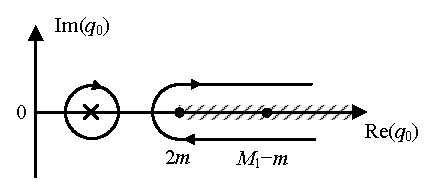
\includegraphics[scale=1.5]{Fig3.eps}
	\caption{Контур интегрирования по $q_0$ в~(\ref{eq:20}) для мод $\lambda = 1,2$. Штриховой линией показана область, где мнимая часть поляризационного оператора двух возможных мод $\lambda = 1,2$ существенна. Остальные обозначения аналогичны~рис.~\ref{fig:FullPathIntegr}.}\label{fig:PathIntegr}
\end{figure}

С учетом процессов излучения фотонов мнимая часть поляризационного оператора может быть представлена в следующей форме (см., например,~\cite{Shabad:1988, Rumyantsev:2017,Weldon:1983}): 
\begin{eqnarray}\label{eq:Ilambda}
I^{(\lambda)}=Im {\cal P}^{(\lambda)} =  -2 q_0 [1-\exp (-q_0/T)] W^{(\lambda)}_{abs} \, . 
\label{eq:ImP}
\end{eqnarray}

Реальная часть поляризационного оператора может быть восстановлена по его мнимой части с помощью дисперсионного соотношения с одним вычитанием:
%
\beq 
R^{(\lambda)}=\textrm{Re}{\cal P}^{(\lambda)} (t) = \int \limits_0^\infty \frac{\textrm{Im}({\cal P}^{(\lambda)} (t'))\,dt'}{t'-t-i o} - \textrm{Re}{\cal P}^{(\lambda)} (0)\,, \qquad  t = q^2_0 \, .
\label{eq:Disp}
\eeq

В общем случае произвольных уровней Ландау $\ell$ и $\ell'$ задача о вычислении $\textrm{Re} {\cal P}^{(\lambda)}(t)$ выглядит очень громоздко, поэтому в сильно замагниченной плазме можно ограничиться вкладом только первых двух уровней Ландау. В~результате выражения для мнимой и действительной частей поляризационного оператора для фотонов моды 1 и моды 2 с учетом~(\ref{eq:Ilambda}--\ref{eq:Disp}) и магнитного поля при условии $q_0^2>4m^2$ удобно представить следующим образом:
\begin{eqnarray}
	\nonumber
		&&I^{(1)}=2\alpha\beta\exp \left[-\frac{q_0^2}{2\beta }\right]\frac{\left(2\beta -q_0^2\right)}{ \sqrt{\left((M_1-m)^2-q_0^2\right) \left((M_1+m)^2-q_0^2\right)}}\times
	\\
	&&\times\left(\frac{1}{\exp\left[\frac{2\beta -q_0^2}{2 q_0 T}\right]+1}-\frac{1}{\exp\left[\frac{2\beta +q_0^2}{2 q_0 T}\right]+1}\right)
\end{eqnarray}

\begin{eqnarray}
		\nonumber
		&&R^{(1)}= -\frac{\alpha \beta}{2\pi}\exp\left[\frac{-q_0^2}{2\beta}\right]\bigg(\frac{M_1^2-m^2-q_0^2}{\sqrt{((M_1+m)^2-q_0^2)((M_1-m)^2-q_0^2)}}
		\times
		\\
		\nonumber
		&&\times
		\ln\left[\frac{\sqrt{(M_1+m)^2-q_0^2}+\sqrt{(M_1-m)^2-q_0^2}}{2\sqrt{M_1 m}}\right]-\ln\left[\frac{M_1^2}{m^2}\right]\bigg)
		-
		\\
		\nonumber
		&&-\frac{\alpha \beta q_0^2 m^2}{2\pi} \exp\left[-\frac{q_0^2}{2\beta}\right]\int_{0}^{\infty}\frac{\dd z}{\exp \left[\frac{m}{T}\sqrt{z^2+1}\,\right]+1}\times
		\\
		&&\times\frac{\sqrt{z^2+1}}{ \left(M_1^2-m^2-q_0^2\right)^2-4m^2q_0^2 \left(z^2+1\right)}\, ,
\end{eqnarray}

\begin{eqnarray}
		\nonumber
		&&I^{(2)}=2\alpha\beta\exp\left[{\frac{-q^2_0}{2\beta}}\right] \bigg\{
		\frac{4 m^2}{q_0\sqrt{q^{2}_{0}-4 m^2}}
	  \left(\frac{1}{\exp\left[\frac{-q_0}{2  T}\right]+1}-\frac{1}{\exp\left[\frac{q_0}{2T}\right]+1}+1\right) +
		\\
		\nonumber
		&&+
		\frac{q_0^2}{2\beta}
		%\times 
		%\\
		%\nonumber
		%&&\times 
		\frac{-4\beta^2/q^{2}_{0} + 2 \beta + 4 m^2}{\sqrt{((M_1+m)^2-q_0^2)((M_1-m)^2-q_0^2)}}\times
		\\
		&&\times\left(\frac{1}{\exp\left[\frac{2\beta -q_0^2}{2 q_0 T}\right]+1}-\frac{1}{\exp\left[\frac{2\beta +q_0^2}{2 q_0 T}\right]+1}+1\right)
		\bigg\}\, ,
\end{eqnarray}

\begin{eqnarray}
\nonumber
		&&R^{(2)}= \frac{\alpha\beta}{2\pi}\exp\left[-\frac{q_0^2}{2\beta}\right]\left(\frac{4m^2}{\sqrt{q_0^2(q_0^2-4m^2)}}\ln\left[\frac{\sqrt{q_0^2}+\sqrt{q_0^2-4m^2}}{4m^2}\right]+1\right)+ 
		\\
		\nonumber
		&&+\frac{\alpha}{16\pi}q^2_0 \exp\left[-\frac{q_0^2}{2\beta}\right] \bigg( \frac{4m^2+2\beta+\frac{4\beta^2}{ q_0^2}}{\sqrt{((M_1-m)^2-q^2_0)((M_1-m)^2-q^2_0)}}
		\times
		\\
		\nonumber
		&&\times
		\ln\left[\frac{\sqrt{(M_1+m)^2-q_0^2}+\sqrt{(M_1-m)^2-q_0^2}}{2(m^4+2\beta m^2)^{1/4}}\right]+
		\\
		\nonumber
		&&+\frac{1}{2}\left(\frac{m^2}{\beta}-\frac{2\beta}{q_0^2}\right)\ln\left[\frac{m^2+2\beta}{m^2}\right]+1\bigg)- \frac{4\alpha\beta m^2}{\pi}\exp\left[-\frac{q_0^2}{2\beta}\right]\times
		\\
		\nonumber
		&&\times
		\int_{0}^{\infty}\frac{1}{\sqrt{1+z^2}}\frac{1}{\exp[\frac{m}{T}\sqrt{(1+z^2)}\,]+1}\bigg(\frac{1}{q_0^2-4m^2(1+z^2)}+
		\\
		&&+\frac{q_0^2}{\beta}\frac{2\beta z^2 + q_0^2}{(2\beta - q_0^2)^2-m^2(1+z^2)q_0^2}\bigg)\dd z\, .
\end{eqnarray}

Следует отметить, что в поставленной задаче рассматриваются процессы только до второго циклотронного резонанса $q_0=M_1-m$, поэтому те же процессы с другими уровнями Ландау вклада не дают.
Выражения (\ref{eq:20})--(\ref{eq:Wabs}) с учетом (\ref{eq:Disp}) решают задачу 
о нахождении временной зависимости волновой функции фотона  в присутствии сильно 
замагниченной плазмы. 

\begin{figure}[t!]\centering
	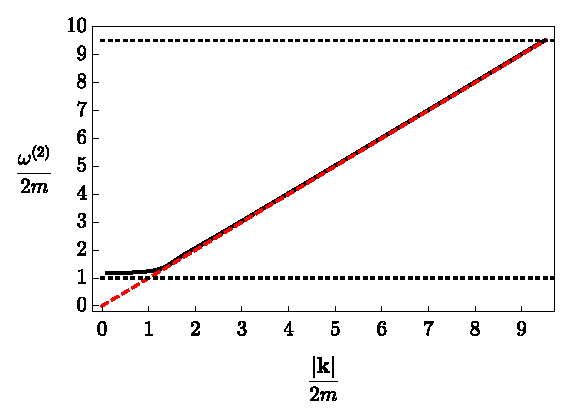
\includegraphics[scale=1.2]{Fig4.eps}
	\caption{Дисперсия фотона моды 2 в области нестабильности, связанной с процессами распада на $e^+e^-$ пару и поглощения $e_0 \gamma^{(2)}\to e_1$, представлена сплошной линией при магнитном поле $B=200B_e$ и $T=1$~МэВ. Штриховая линия соответствует вакуумному закону дисперсии. Пунктирные линии обозначают пороги $\omega^{(2)}=2m$ и $\omega^{(2)}=M_1-m$. \label{fig:DisperseMode2}}
\end{figure}

Временную часть волновой функции фотона $F(t)$ можно представить в виде затухающих колебаний для мод $\lambda=1,2$:
\begin{equation}\label{eq:Fm}
	F^{(\lambda)}(t)\sim F^{(\lambda)}_A(t) \cos(\omega^{(\lambda)} t+\phi_0)
\end{equation}
где $F^{(\lambda)}_A(t)$ -- амплитуда колебаний,
временная зависимость которой определяет
характер затухания волновой функции,
$\omega^{(\lambda)}$ -- эффективная
частота. В работе~\cite{Shabad:1988}
предполагался экспоненциальный характер затухания с декрементом затухания, равным мнимой части энергии фотона, полученным из решения уравнения дисперсии на втором римановом листе. Рассмотрение  аналитических свойств фурье-образа $F^{(\lambda)}_{cut}(q_0)$ показывает, что характер временного затухания волновой функции в общем случае является неэкспоненциальным. Тем не менее на протяжении некоторого характерного отрезка времени $(\sim [W^{(\lambda)}_{abs}]^{-1})$
зависимость волновой функции от времени можно приближенно описать как 
экспоненциально затухающие гармонические колебания:
%
\begin{equation}\label{eq:ApproxA}
{\cal A}^{(\lambda)}_\mu(t) \sim e^{- \gamma^{(\lambda)}_{eff} \, t/2} \cos 
(\omega^{(\lambda)} t + \phi_0).
\end{equation}
%
Здесь $\omega^{(\lambda)}$ и $\gamma^{(\lambda)}_{eff}$ -- эффективная 
частота и коэффициент  
поглощения фотона моды $\lambda$ соответственно, которые должны быть найдены с использованием 
(\ref{eq:20})--(\ref{eq:Wabs}) для каждого значения импульса ${\bf k}$, что определяет эффективный 
закон дисперсии фотона в области его нестабильности~(см. рис.~\ref{fig:DisperseMode1} и \ref{fig:DisperseMode2}).


%%%%%%%%%%%%%%%%%%%%%%%%%%%%%%%%%%%%%%%%%%%%%%%%%%%%%%%%%%%%%%%%%%%%%%%%%%%%%%%%%%%%%%%%%%%%%%%%%%%%%%%%%%%%%%%%%%%%%%%%%%%%%%%%%%%%%%%%%%%%%%%%%%%%%%%%%%%
\section{Численный анализ}




\begin{figure}[t]\centering
	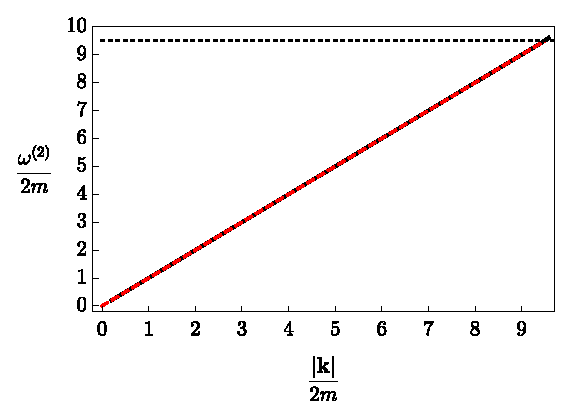
\includegraphics[scale=1]{Fig5.eps}
	\caption{Дисперсия фотона моды 1 в области нестабильности, связанной с процессом поглощения $e_0 \gamma^{(1)}\to e_1$ представлена при магнитном поле $B=200B_e$ и $T=1$~МэВ. Пунктирная линия обозначает порог $\omega^{(1)}=M_1-m$ \label{fig:DisperseMode1}}
\end{figure}

Рис.~\ref{fig:DisperseMode1} и ~\ref{fig:DisperseMode2} демонстрируют законы дисперсии фотонов моды 1 и моды~2 в сильно замагниченной плазме при температуре $T = 1$ МэВ и магнитном поле $B = 200B_e$ в области их нестабильности. Из представленных результатов следует, что закон дисперсии для фотона моды 1 в области нестабильности незначительно отличается от вакуумного закона дисперсии~(см.~рис.~\ref{fig:DisperseMode1}). С другой стороны, дисперсионная кривая фотона моды 2 значительно отличается от вакуумной вблизи порога $\omega^{(2)}=4m$ и в малой окрестности порога~$\omega^{(2)}=M_1-m$. Для построения дисперсионной кривой до следующего резонанса необходимо учитывать следующие уровни Ландау. При этом полученная картина дисперсионных кривых согласуется с анализом уравнения дисперсии, выполненного в работе~\cite{Shabad:1988}.


\begin{figure}[t]\centering
	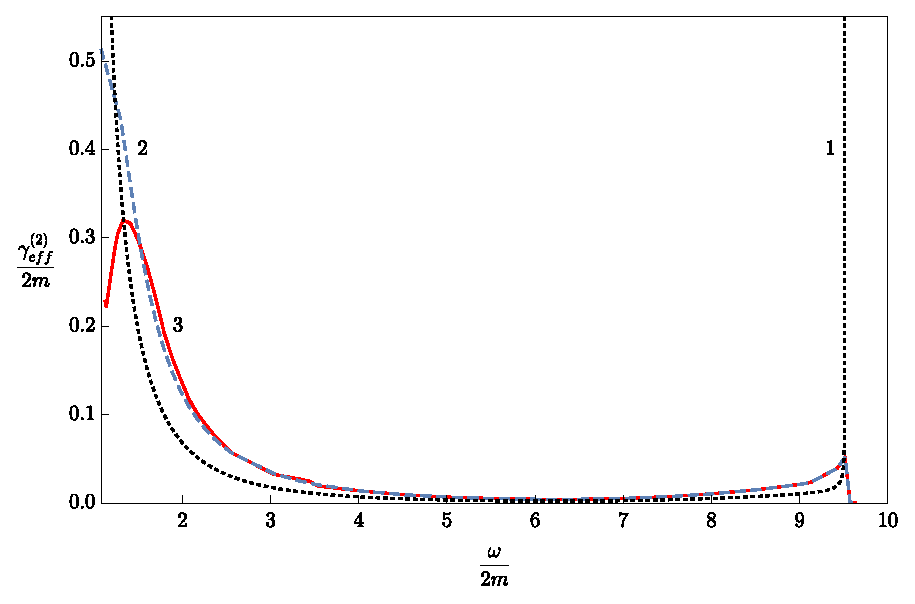
\includegraphics[scale=1]{Fig6.eps}
	\caption{\label{fig:fig2}Зависимость ширины распада фотона моды 2 от частоты в припороговых областях при $B=200 B_e$, $T=1$ МэВ и $ \mu=0 $. Линия $ {\it 1} $ - коэффициент поглощения фотона $ W ^ {(1)}_{abs} $,
		вычисленный в древесном приближении и содержащий корневые особенности; линия $ {\it 2} $ - ширина распада, полученная из комплексного решения дисперсионного уравнения на втором римановом листе [6]; линия $ {\it 3} $ соответствует ширине затухания $ \gamma^{(1)}$, вычисленной на основе приближения~(\ref{eq:ApproxA}).}\label{fig:DampMode2}
\end{figure}

Для астрофизических приложений полезно вычислить величину $\gamma_{eff}$, которая определяет интенсивность поглощения 
$\gamma$-квантов в замагниченной плазме за счет  процессов $\gamma \to e^+ e^-$  и $\gamma e^{\pm} \to e^{\pm}$.
Обычно в астрофизике  используют выражение для коэффициента поглощения,
полученное на основе  вероятности распада  $ \gamma \to e^+ e^-$. Однако в околопороговой области эти выражения
содержат корневые сингулярности (см. например~\cite{HBG:1997}). 

На рисунках \ref{fig:DampMode2} 
и~\ref{fig:DampMode1} представлен коэффициент поглощения фотона в зависимости 
от эффективной частоты, определенный исходя из результатов~\cite{Shabad:1988,HBG:1997} и результаты данной работы. Наш анализ показывает,
что вычисление коэффициента  поглощения с учетом неэкспоненциального характера 
затухания приводит к конечному выражению для коэффициента  поглощения фотона в окрестности резонансов 
$q_0 = (\sqrt{m^2+2 \beta} - m )$ как для фотона моды 2, так и для фотона моды 1. Исходя из рис. \ref{fig:DampMode1} можно сделать вывод, что фотон моды 1 является квазистабильным в областях $q_0<7$ МэВ и $q_0>(\sqrt{m^2+2 \beta} - m)\simeq 9.5$~МэВ. С другой стороны, фотон неустойчив в области, близкой в окрестности резонансов $q_0 = (\sqrt{m^2+2 \beta} - m )$. Фотон моды 2 можно считать квазиустойчивым в области $q_0<4m$ и $q_0>(\sqrt{m^2+2 \beta} - m)$. Коэффициент затухания фотона, полученный из результатов работы~\cite{Shabad:1988}, является завышенным в околопороговой области по сравнению с результатами, полученными с помощью аппроксимации~(\ref{eq:ApproxA}). Однако существует область энергий фотона ($2.5\lesssim q_0\lesssim 8.5$ МэВ для фотона моды 2 и $q_0\lesssim8.7$ МэВ для фотона моды 1), где коэффициенты поглощения, полученные из результатов работы~\cite{Shabad:1988} и с помощью аппроксимации~(\ref{eq:ApproxA}) совпадают.


\begin{figure}[t]\centering
	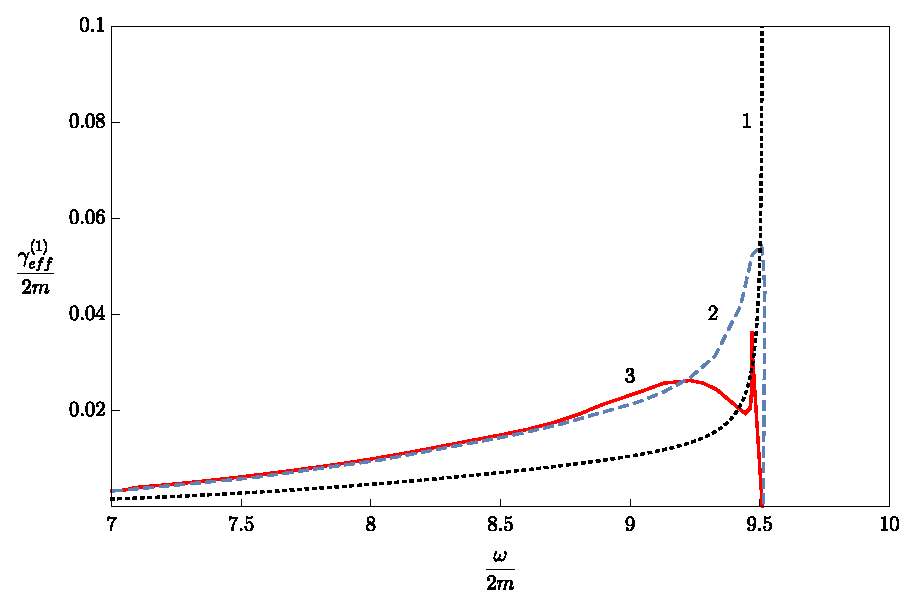
\includegraphics[scale=0.6]{Fig7.eps}
	\caption{\label{fig:fig1}Зависимость ширины распада фотона моды 1 от частоты в припороговых областях при $B=200 B_e$, $T=1$ МэВ и $ \mu=0 $. Линия $ {\it 1} $ - коэффициент поглощения фотона $ W ^ {(1)}_{abs} $,
		вычисленный в древесном приближении и содержащий корневые особенности; линия $ {\it 2} $ - ширина распада, полученная из комплексного решения дисперсионного уравнения на втором римановом листе [6]; линия $ {\it 3} $ соответствует ширине затухания $ \gamma^{(1)}$, вычисленной на основе приближения~(\ref{eq:ApproxA}).}\label{fig:DampMode1}
\end{figure}

\begin{figure}[t!]\centering
	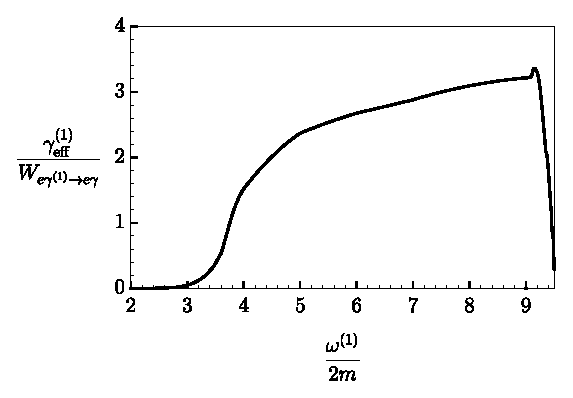
\includegraphics[scale=1.3]{Fig8.eps}
	\caption{\label{fig:ComptonandDamp} Отношение коэффициента затухания фотона $\gamma_{eff}^{(1)}$ к коэффициенту поглощения фотона в процессе $e\gamma^{(1)}\to e\gamma$ при $B=200B_e$ и $T=1$ МэВ}
\end{figure}
\begin{figure}[t!]\centering
	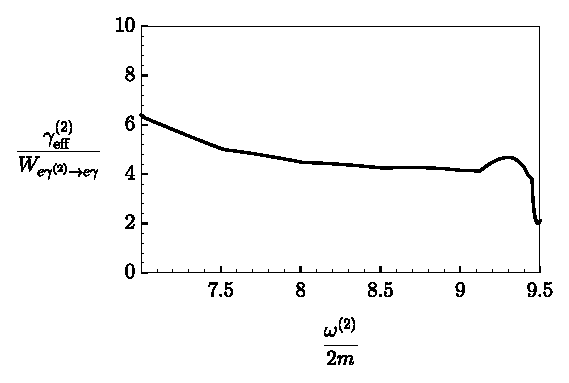
\includegraphics[scale=1.3]{Fig9.eps}
	\caption{\label{fig:ComptonandDamp2} Отношение коэффициента затухания фотона $\gamma_{eff}^{(2)}$ к коэффициенту поглощения фотона в процессе $e\gamma^{(2)}\to e\gamma$ при $B=200B_e$ и $T=1$ МэВ}
\end{figure}
\clearpage

На основе полученных результатов представляет интерес рассмотреть задачу о возможности формирования комптоновского процесса при условии затухания фотона. Для этого удобно вычислить отношение коэффициента затухания фотона к коэффициенту поглощения фотона $e\gamma^{(1)}\to e\gamma$  (см. рис. \ref{fig:ComptonandDamp}), полученному работе~\cite{JETP2026}, определяющему время его формирования. Как видно из рисунка~\ref{fig:ComptonandDamp}, комптоновский процесс, несмотря на малый фактор $\alpha$, успевает формироваться при энергиях фотона $\omega\lesssim3$ МэВ. Для фотона моды 2 комптоновский процесс формируется только в области энергий фотона $\omega\lesssim1$ МэВ. В области энергий $\omega>3$ МэВ для моды 1 и $\omega>1$ МэВ фотоны будут эффективно затухать, и комптоновский процесс, по-видимому, не успевает сформироваться. Для моды 2 (см. рис.~\ref{fig:ComptonandDamp2}) даже с учетом области квазистабильности (вдали от порогов), комптоновский процесс будет формироваться только при энергиях фотона~$\omega<1$~МэВ.

Таким образом, коэффициенты поглощения фотона в комптоновском процессе для двух возможных каналов рассеяния $e\gamma^{(1)}  \to e\gamma^{(1)}$ и $e\gamma^{(1)}  \to e\gamma^{(2)}$, несмотря на резонансный характер, целесообразно рассматривать лишь вдали от циклотронных резонансов, поэтому для анализа комптоновского процесса при высоких температурах $T\simeq 1$ МэВ и магнитных полях $B=200 B_e$ достаточно использовать разложение по обратным степеням напряженности магнитного поля~\cite{Chistyakov:2009}. Каналы же рассеяния $e\gamma^{(2)}  \to e\gamma^{(1)}$  и $e\gamma^{(2)}  \to e\gamma^{(2)}$ в области резонанса рассматривать нецелесообразно, так как комптоновский процесс не успевает сформироваться для энергий фотона $\omega\gtrsim 2m$.
%%%%%%%%%%%%%%%%%%%%%%%%%%%%%%%%%%%%%%%%%%%%%%%%%%%%%%%%%%%%%%%%%%%%%%%%%%%%%%%%%%%%%%%%%%%%%%%%%%%%%%%%%%%%%%%%%%%%%%%%%%%%%%%%%%%%%%%%%%%%%%%%%%%%%%%%%%%
\section{Заключение}

Исследован процесс распространения квантованной электромагнитной волны в сильно замагниченной, зарядово-симметричной плазме. С учетом изменения дисперсионных свойств фотона в магнитном поле и плазме было установлено, что, аналогично случаю чистого магнитного поля процесс затухания фотона
в замагниченной плазме имеет неэкспоненциальный характер. 

Для характерного отрезка времени $\sim [W^{{(\lambda)}}_{abs}]^{-1}$ была использована аппроксимация экспоненциально затухающими колебаниями. В этом случае было
показано, что коэффициент поглощения фотона в околопороговой области меньше по сравнению с известными в литературе результатами. Также, следуя данной аппроксимации, были построены дисперсионные кривые, которые и для моды 1, и для моды 2 близки к вакуумным кривым, за исключением околопороговых областей. Полученные результаты согласуются с выводами работы~\cite{Shabad:1988}.

Кроме того, был выполнен анализ возможности формирования комптоновского процесса в условиях нестабильности фотона за счет процесса поглощения электроном $e^\pm\gamma\to e^\pm$ и распада на электрон-позитронную пару $\gamma\to e^+e^-$. Несмотря на малый фактор $\alpha$, комптоновский процесс преобладает над процессами распада и поглощения в области низких энергий фотона ($\omega<3$ МэВ при $T=1$ МэВ и $B =200B_e$). С другой стороны, даже с учетом резонанса на виртуальном электроне, фотоны как моды 1, так и моды~2 в пределе сильного магнитного поля $B=200 B_e$ и температуре $T=1$ МэВ эффективно затухают в резонансной области.

Для определения характера затухания фотона необходимо выполнить более детальный анализ временной зависимости амплитуды $F_A(t)$ колебаний, входящей в уравнение~(\ref{eq:Fm}).

%%%%%%%%%%%%%%%%%%%%%%%%%%%%%%%%%%%%%%%%%%%%%%%%%%%%%%%%%%%%%%%%%%%%%%%%
%% Библиография %%%%%%%%%%%%%%%%%%%%%%%%%%%%%%%%%%%%%%%%%%%%%%%%%%%%%%%%
%%%%%%%%%%%%%%%%%%%%%%%%%%%%%%%%%%%%%%%%%%%%%%%%%%%%%%%%%%%%%%%%%%%%%%%%

\begin{thebibliography}{}
\bibitem{KuznMikh}
Kuznetsov A., Mikheev N. Electroweak processes in external active media //
Springer Tracts Mod. Phys. 2013. Vol. 252. 271 p.
%
\bibitem{Klepikov:1954}
Клепиков Н. П. Излучение фотонов и электрон-позитронных пар в магнитном
поле // Журнал экспериментальной и теоретической физики. 1954.
Т. 26, № 1. С. 19–34.
%
\bibitem{Sturrock:1971}
Sturrock C. A. A model of pulsars // Astrophys. J. 1971. Vol. 164. P. 529–556.
%
\bibitem{Daugherty:1983}
Daugherty J. K. Pair production in superstrong magnetic fields // Astrophys.
J. 1983. Vol. 273. P. 761–773.
%
\bibitem{Shabad:1988}
Шабад А. Е. Поляризация вакуума и квантового релятивистского газа во
внешнем поле // Тр. ФИАН СССР. 1988. Т. 192. С. 5–152.
%
\bibitem{Tademaru:1973}
Tademaru E. On the energy spectrum of relativistic electrons in the crab nebula
// Astrophys. J. 1973. Vol. 183. P. 625–635.
%
\bibitem{Baier:2007}
Baier V. N., Katkov V. M. Pair creation by a photon in a strong magnetic
field // Phys. Rev. D. 2007. Vol. 75, no. 7. P. 073009.
%
\bibitem{Landau:1946}
Ландау Л. Д. О колебаниях электронной плазмы // Успехи физических
129 наук. 1946. Vol. 93, no. 3. P. 527–540.
%
\bibitem{MikhChist:2001}
Михеев Н. В., Чистяков М. В. Затухание фотона в результате рождения
электрон-позитронной пары в сильном магнитном поле // Письма в
Журнал экспериментальной и теоретической физики. 2001. Т. 73, № 12.
С. 726–730.
%
\bibitem{Kirzhnits:1987}
Киржниц Д. А. Общие свойства электромагнитных функций отклика //
Успехи физических наук. 1987. Vol. 152, no. 7. P. 399–422.
%
\bibitem{Landau:2001}
Ландау Л. Д., Лифшиц Е. М., Питаевский Л. П. Теоретическая физика:
ч. 2. Статистическая физика. Теория конденсированного состояния. ФИЗМАТЛИТ,
2001. Т. IX. 496 с.
%
\bibitem{Tsai:1974}
Tsai W. Y. Vacuum polarization in homogeneous magnetic fields // Phys.
Rev. D. 1974. Vol. 10, no. 8. P. 2699–2702.
%
\bibitem{Batalin:1971}
Баталин И. А., Шабад A. E. Функция Грина фотона в постоянном однородном
электромагнитном поле общего вида // Журнал экспериментальной
и теоретической физики. 1971. Т. 60, № 3. С. 894–900.
%
\bibitem{Skobelev:1975}
Скобелев В. В. Поляризационный оператор фотона в сверхсильном магнитном
поле // Изв. вузов. Физика. 1975. № 10. С. 142–143.
%
\bibitem{Rumyantsev:2017}
Румянцев Д. А., Шленев Д. М., Ярков А. А. Резонансы в комптоноподобных
процессах рассеяния во внешней замагниченной среде // Журнал экспериментальной
и теоретической физики. 2017. Т. 152, № 3. С. 483–494.
%
%
\bibitem{Gradshteyn} 
Gradshteyn, I. S. Table of Integrals, Series, and Products / I.~S.~Gradshteyn, I.~M.~Ryzhik. -- Academic, New York, 1980.
%
\bibitem{Weldon:1983}
Weldon H. A. Simple rules for discontinuities in finite temperature field theory
// Phys. Rev. D. 1983. Vol. 28. P. 2007–2037.
%
\bibitem{HBG:1997}
Harding A. C., Baring M. G., Gonthier P. L. Photon splitting cascades in
Gamma-Ray pulsars and the spectrum of PSR1509-58 // Astrophys. J. 1997.
Vol. 476. P. 246–260.
%
\bibitem{Chistyakov:2009}
Chistyakov M. V., Rumyantsev D. A. Compton effect in strongly magnetized
plasma // Int. J. Mod. Phys. 2009. Vol. A24. P. 3995–4008.
%
\bibitem{JETP2026}
Румянцев Д. А., Ярков А. А., Шленев Д. М. Резонансное комптоновское рассеяние в замагниченной среде // Журнал экспериментальной
и теоретической физики. 2026. Т. ?, № ?. С. ?.
\end{thebibliography}

\end{document}






